\chapter{Petalinux} \label{ch:petalinux}
Petalinux is an embedded Software Development Kit - SDK - targeting FPGA-based System on a Chip - SoC - design or FPGA designs.


\section{Installation procedure}
Before the actual installation of Petalinux SDK, the creation of a compatible environment is requested.
There are few steps to be followed in order to configure such environment:
\begin{itemize}
	\item Adding the 32-bit architecture to the system
	\item Installing all the required packages for the Petalinux Build Host 
\end{itemize}

\subsection{i386 architecture}
The 32bit architecture is essential for Petalinux to be installed. To add such architecture to the system, open the command prompt and type the following command:
\begin{verbatim}
	$ sudo dpkg --add-architecture i386
\end{verbatim}
It is now possible to check the availability of the architecture by typing
\begin{verbatim}
	$ dpkg --print-foreign-architectures
\end{verbatim}
and an output similar to that of Figure \ref{fig:i386} will appear.
\begin{figure}[ht]
	\centering
	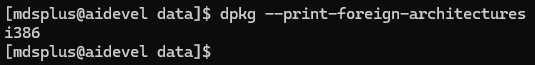
\includegraphics[width=0.7\textwidth]{images/i386}
	\caption{Successful installation of i386 architecture.}
	\label{fig:i386}
\end{figure}

\subsection{Petalinux Build Host packages}
From this \href{https://adaptivesupport.amd.com/s/article/73296?language=en_US}{page}, download the file at the bottom. Create the folder in which petalinux will be installed with the command \begin{verbatim}
	mkdir <folder_name>
\end{verbatim}
and copy the file from the download folder to the this final folder. Within this example, such folder is named ptlnx. To start the installation of all the packages type 
\begin{verbatim}
	chmod +x <installer_file_name>
	sudo ./<file_name>
\end{verbatim}
Once the installation is complete, all the packages should have been installed.

\subsection{Petalinux SDK installation}
Now it is possible to begin the actual installation of Petalinux. From the \href{https://www.xilinx.com/support/download/index.html/content/xilinx/en/downloadNav/embedded-design-tools/archive.html}{AMD download page}, download the needed version and move it to the installation folder. From this page also download the .BPS file relative to the board to be used. This latter file has to be moved into the folder in which the petalinux project are saved. Now type
\begin{verbatim}
	chmod +x <installer_file_name>
	./<file_name>
\end{verbatim}
Now the installation should begin. By following the instruction, the installation process should proceed without any inconvenience, even though it might take a while. Finally, to set the Petalinux environment into the directory in which it is installed, type
\begin{verbatim}
	source settings.sh
\end{verbatim}
from which the shell output is highlighted in Fig. \ref{fig:pt1} is shown. Now the system should be all set.
\begin{figure}[ht]
	\centering
	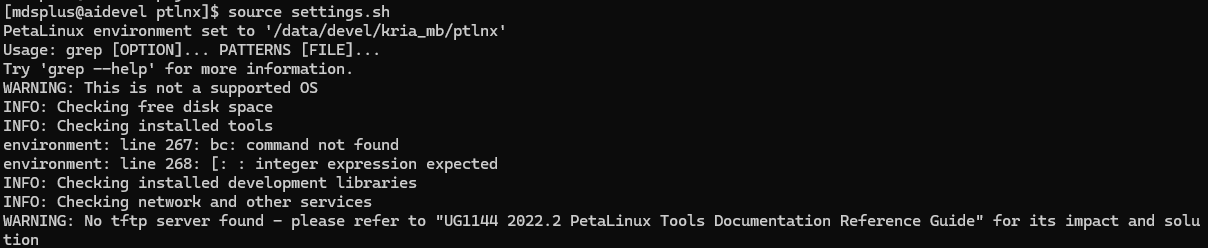
\includegraphics[width=\textwidth]{images/pt1}
	\caption{Setting petalinux environment.}
	\label{fig:pt1}
\end{figure}
